\documentclass[prb,papersize=a4paper,notitlepage]{revtex4-1}%
\usepackage{hyperref}
\usepackage{enumitem}
\usepackage{nicefrac}
\usepackage{amsmath}
\usepackage{graphicx}
\usepackage{amsfonts}
\usepackage{physics}
\usepackage{amssymb}
\usepackage{bm}
\usepackage[utf8]{inputenc}
\usepackage[russian]{babel}
\usepackage{listings}


\begin{document}

\title{Вычислительная физика, Осень 2020 ВШЭ. Задание 5.\footnote{Дополнительно указаны: (количество баллов за задачу)[имя задачи на nbgrader]}}
\maketitle
\begin{enumerate}
\item \textbf{Восстановление зашумлённого изображения (30)} Скачайте \href{https://www.dropbox.com/s/qgz1x67t10fd7hf/data.npz?dl=0}{файл}, содержащий матрицы $A$ и $C$ (изображение и фильтр) и откройте его, используя \lstinline{numpy}:
\lstset{language=Python}
\lstset{frame=lines}
\lstset{label={lst:code_direct}}
\lstset{basicstyle=\ttfamily}
\begin{lstlisting}
with np.load('data.npz') as data:
    A, C = data['A'], data['C']
\end{lstlisting}
Для работы с изображением нам будет удобно выстраивать элементы матрицы $A$ в вектор--столбец $a$:
\lstset{language=Python}
\lstset{frame=lines}
\lstset{label={lst:code_direct}}
\lstset{basicstyle=\ttfamily}
\begin{lstlisting}
def mat2vec(A):
    h, w = A.shape
    a = np.zeros(h*w, dtype=A.dtype)
    A = np.flipud(A) 
    for i, row in enumerate(A):
        a[i*w:i*w+w] = row
    return a
\end{lstlisting}
так что обратное преобразование -- от вектора $a$ в матрицу $A$ осуществляется с помощью функции
\lstset{language=Python}
\lstset{frame=lines}
\lstset{label={lst:code_direct}}
\lstset{basicstyle=\ttfamily}
\begin{lstlisting}
def vec2mat(a, shape):
    h, w = shape
    A = np.zeros(shape, dtype=a.dtype)
    for i in range(h):
        A[i, :] = a[i*w:i*w+w]
    return np.flipud(A)
\end{lstlisting}
Изображение, содержащееся в матрице $A$ получено из некоторого оригинала $A_0$ путем свёртки его с фильтром $C$ и добавлением шума. Фильтр $C$ осуществляет `размытие' изображения, одновременно меняя его размер от $16\times 51$ к $25\times 60$. Используя соответствующие вектора $a$ и $a_0$, эту операцию можно записать так
$$
a_0\to a = C a_0 + \epsilon,
$$
где $\epsilon$ - вектор, состоящий из нескоррелированных случайных величин из нормального распределения. Ваша задача состоит в том, чтобы располагая зашумленным изображением $A$ и фильтром $C$, восстановить исходное изображение $A_0$.
\begin{figure}[h!]
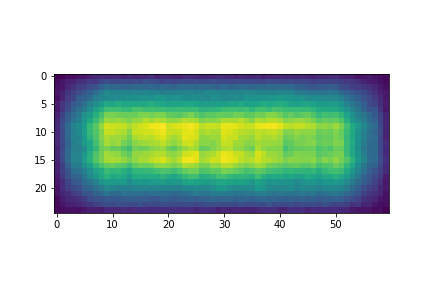
\includegraphics[width=8cm]{im.png}
\caption{Изображение $A$.}
\label{subs}
\end{figure}
\begin{itemize}
\item Постройте изображение, содержащееся в $A$ (у вас должен получиться Рис. 1).
\item Исследуйте действие фильтра $C$ на изображения: составьте (на свой выбор) матрицу, и проверьте, что с соответствующим изображением делает фильтр $C$. Вам понадобятся операции \lstinline{a = mat2vec(A)} и \lstinline{A0 = vec2mat(a0, shape)} для перехода от матричного к векторному представлению и обратно.
\item Наивный способ восстановить изображение $A_0$ по изображению $A$ состоит в том, чтобы решить систему $a = C a_0$ относительно вектора $a_0$. Какой является эта система: недо-- или переопределённой? Используйте SVD матрицы $C$ чтобы найти $a_0$ и постройте соответствующее изображение $A_0$.
\item Для того, чтобы улучшить результат, поэкспериментируйте с количеством удержанных собственных значений при решении системы уравнений в предыдущем пункте. Что находится на изображении $A_0$?
\end{itemize}
\item \textbf{Ранжирование веб--страниц (35)} Одна из самых известных задач о вычислении собственных векторов -- задача о ранжировании $n$ веб-страниц. Подход, который вам нужно будет реализовать в этой задаче, был одним из главных в работе Google на раннем этапе. Всё, что мы собираемся использовать -- структуру взаимных ссылок между страницами. \lstinline{PageRank} определяется рекурсивно: важность $i$--й страницы определяется как среднее значение важностей всех страниц, которые ссылаются на $i$--ю. Обозначим важность $i$--й страницы $p_i$, тогда это определение может быть записано в виде линейной системы:
$$ p_i = \sum_{j} \frac{p_j}{L(j)}l_{ij}, $$
где $l_{ij}=1$ если $j$--я страница ссылается на $i$--ю (в противном случае $l_{ij}=0$), а $L(j)$ -- количество исходящих ссылок со страницы $j$. Система может быть переписана в виде задачи на собственное значение:
$$ p = G p, \quad G_{ij} = \frac{l_{ij}}{L(j)}.$$ Если в графе есть `подвешенные' узлы (все элементы какого-то столбца равны нулю), то весь столбец заполняется числом $1/n$. Наконец, вводится параметр $0<\beta<1$ так что матрица $G$ заменяется на
$$
G\to \beta G + \frac{1-\beta}{n} e e^T,
$$
где $e$ -- вектор, состоящий из единиц. Обратите внимание, что задача свелась к нахождению собственного вектора $p$ матрицы $G$, отвечающего собственному значению 1.  Можно показать [*], что  1 -- максимально возможное собственное значение матрицы $G$.

\begin{itemize}
\item Придумайте самостоятельно небольшой граф связности ($~10$ узлов), постройте соответствующие матрицы $l$ и $G$ и найдите численно собственный вектор, отвечающий \lstinline{PageRank}.
\item Скачайте \href{http://snap.stanford.edu/data/web-Stanford.txt.gz}{файл}, в котором представлен ориентированный граф, узлы которого составляют страницы stanford.edu, а направленные рёбра -- ссылки между ними (граф задан матрицей смежности $l$). Распакуйте архив и загрузите его:
\lstset{language=Python}
\lstset{frame=lines}
\lstset{label={lst:code_direct}}
\lstset{basicstyle=\ttfamily}
\begin{lstlisting}
from scipy import sparse
def dataset2csr(filename, nodes, edges):
    rows = []; cols = []    
    with open(filename, 'r') as f:
        for line in f.readlines()[4:]:
            o, d = (int(x)-1 for x in line.split())
            rows.append(d)
            cols.append(o)
    return(sparse.csr_matrix(([True]*edges, (rows, cols)), shape=(nodes, nodes)))

l = dataset2csr(filename='web-Stanford.txt', nodes = 281903, edges=2312497)
\end{lstlisting}
\item Найдите \lstinline{PageRank} для матрицы из предыдущего пункта. Для этого реализуйте степенную итерацию для нахождения собственного вектора, отвечающего максимальному собственному значению $G$. Возьмите $\beta = 0.8$.
\item Итерируйте до тех пор, пока 1--норма изменения вектора-кандидата не станет меньше $10^{-4}$. Сколько итераций понадобилось?
\item Какому собственному значению отвечает найденный вектор и у какого узла наибольший \lstinline{PageRank}? 
\item Докажите утверждение (*).
\end{itemize}


\item \textbf{Одномерный кристалл (30)} Рассмотрите одномерный кристалл с двумя атомами различной массы $m$ и $M$ в элементарной ячейке, состоящий из $N$ элементарных ячеек (всего $2N$ атомов), замкнутых в кольцо (периодические граничные условия).  
\begin{itemize}
\item Считая, что соседние атомы на кольце соединены одинаковыми пружинами c упругой константой $k=1$, выпишите уравнения движения (уравнения Ньютона) на положения атомов $x_i$. 
\item Предполагая, что все атомы движутся с одной и той же частотой, $x_i(t)=u_i e^{-i\omega t}$, перепишите найденные выше уравнения в виде системы линейных уравнений на вектор $u$. Составьте матрицу $A$, спектр которой определяет частоты нормальных мод.
\item Используя \lstinline{np.linalg.eig}, найдите спектр матрицы $A$ (возьмите $N = 1000$ и $M/m = 2$). Постройте гистограмму собственных значений. Обратите внимание, что в спектре есть щель -- `запрещенная'  область энергии внутри спектра, которая разделяет `разрешенную' область на две части.
\item Пострайте пространственную структуру численно определённой нормальной моды $u_i$ вблизи минимальной и максимально энергий спектра. 
\item Теперь рассмотрите цепочку со случайным $k$, взятым из однородного распределения на отрезке $\left[1, 10\right]$ и $M/m = 2$. Найдите её спектр (постройте гистограмму) и изобразите пространственную структуру какой--то моды $u$ из середины спектра.
\end{itemize}
\end{enumerate} 
\end{document}